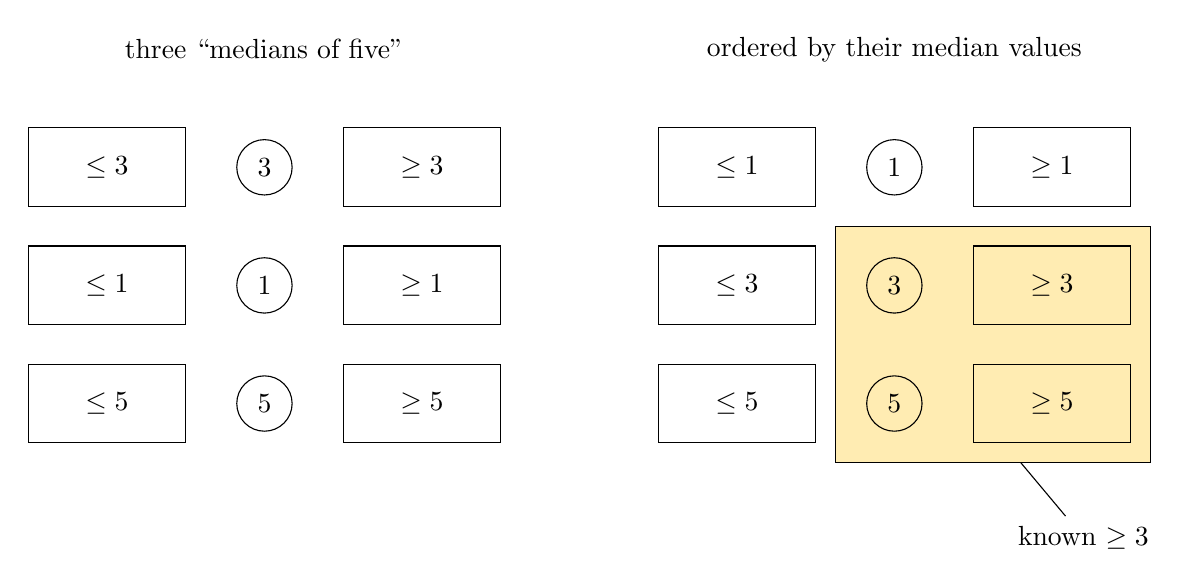
\begin{tikzpicture}
\definecolor{amber}{rgb}{1.0, 0.75, 0.0}

\draw [fill=amber, fill opacity=0.3] (7.25,3.75) rectangle (11.25,0.75);

\draw  (-3,5) rectangle (-1,4);
\node [shape=circle, draw=black, minimum size=2em] at (0,4.5) {3};
\draw  (1,5) rectangle (3,4);
\draw  (-3,3.5) rectangle (-1,2.5);
\draw  (1,3.5) rectangle (3,2.5);
\draw  (-3,2) rectangle (-1,1);
\draw  (1,2) rectangle (3,1);
\node [shape=circle, draw=black, minimum size=2em] at (0,3) {1};
\node [shape=circle, draw=black, minimum size=2em] at (0,1.5) {5};
\node at (0,6) {three ``medians of five"};
\node at (-2,4.5) {$\leq 3$};
\node at (2,4.5) {$\geq 3$};
\node at (-2,3) {$\leq 1$};
\node at (2,3) {$\geq 1$};
\node at (-2,1.5) {$\leq 5$};
\node at (2,1.5) {$\geq 5$};
\node at (4,3) {$\implies$};
\draw  (5,5) rectangle (7,4);
\draw  (9,5) rectangle (11,4);
\draw  (5,3.5) rectangle (7,2.5);
\draw  (9,3.5) rectangle (11,2.5);
\draw  (5,2) rectangle (7,1);
\draw  (9,2) rectangle (11,1);
\node [shape=circle, draw=black, minimum size=2em] at (8,4.5) {1};
\node [shape=circle, draw=black, minimum size=2em] at (8,3) {3};
\node [shape=circle, draw=black, minimum size=2em] at (8,1.5) {5};
\node at (8,6) {ordered by their median values};
\node at (6,4.5) {$\leq 1$};
\node at (10,4.5) {$\geq 1$};
\node at (6,3) {$\leq 3$};
\node at (10,3) {$\geq 3$};
\node at (6,1.5) {$\leq 5$};
\node at (10,1.5) {$\geq 5$};
\node (v1) at (10.4,-0.2) {known $\geq 3$};
\node (v2) at (9.5,0.875) {};
\draw  (v1) edge (v2);
\end{tikzpicture}